\documentclass{IOS-Book-Article}
\usepackage[utf8]{inputenc}
\usepackage{graphicx}
\usepackage{framed}


\def\hb{\hbox to 11.5 cm{}}

\newcommand{\sembrack}[1]{[\![#1]\!]}
\newcommand{\subex}[2]{#1_{#2}}
\newcommand{\commentOut}[1]{}
\newcommand{\eop}[1]{\mbox{\textsl{#1}}}
\newcommand{\ttop}[1]{\mbox{\texttt{#1}}}

\newcommand{\bequ}{\begin{quote}}
\newcommand{\enqu}{\end{quote}}
\newcommand{\bece}{\begin{center}}
\newcommand{\ence}{\end{center}}
\newcommand{\todoj}[1]{{\color{red}\textbf{[J: #1]}}}


\newenvironment{compactitem}{\begin{itemize}}{\end{itemize}}

\begin{document}

\pagestyle{headings}
\def\thepage{}
\begin{frontmatter}              % The preamble begins here.

\title{An End-to-End Pipeline from Law Text to Logical Formulas}

\markboth{}{August 2022\hb}

\author[A]{Aarne Ranta}
\author[C]{Inari Listenmaa}
\author[C]{Jerrold Soh}
\author[C]{Meng Weng Wong}

\address[A]{
  Department of Computer Science and Engineering,
  Chalmers University of Technology and University of Gothenburg,
  aarne.ranta@cse.gu.se
  }
\address[B]{SMU and Digital Grammars}
\address[C]{Yong Pung How School of Law, Singapore Management University}
% \address[D]{Yong Pung How School of Law, Singapore Management University}

\begin{abstract}
This paper describes an experimental pipeline starting from ordinary English law text, parsing it with a formal grammar, and converting it to logical formulas via a series of structural representations.
The goal is to see how to cover the full pipeline with a sequence of well-understood rule-based steps.
The approach is outside-in: we wanted to deliver some output from day 1, and refined it as we went on.
Thus it is a rule-based robust approach.
%%
The law text addressed is one chapter of law of Singapore, Part 6A of the Personal Data Protection Act 2012.
While more work is needed to port the method to other law texts, we believe to have achieved a reusable modular structure, as well as some reusable code, for a more general pipeline.
The pipeline includes some new methods and concepts, in particular, annotation-based grammar writing and an assembly logic for two-dimensional spreadsheet representations.
The code is available as open source.
\end{abstract}


\begin{keyword}
parsing law text
\end{keyword}
\end{frontmatter}
\markboth{August 2022\hb}{August 2022\hb}

%\maketitle
% \section{Relevant LIT and notes}

% Valente and Breuker 1991 - interpretation models or abstract configurations of reasoning steps (e.g. steps we follow in diagnosis) - identifies interpretation of law as one key problem - so already in fields founding we know of the problem - most typical task in legal is assessment: is X  the case? - differs from other domains because contains high degree of common sense reasoning n (1) identifying category membership (and open categories = open texture, which should be human resolved) and (2) come to a coherent interpretation of regulations, make bridging inferences that allow one to understand a rule as exception or related to another, etc -- idea of law functions from Bertalanffy's general system theory -- law exists to accomplish some internal and externals functions, and these objectives reflect on the legal instruments that interact wider society and legal system (being regulations, etc) -- basic set of law functions include: definitions, normativity (saying such and such is illegal), reaction (punishment or reward), creation (creating an entity), prescription (advice to agents). Each implies their own set of domain structures (rules and mechanisms) and inference steps (analysis actions, such as classify, specific, control)

% Haan 1992 - describes how expressing just 2 paras of Dutch traffic regulations in formal logic already exposed situations legislators did not consider (or rather took for granted given their world knowledge), and suggests ways around it. For example, rule says motorbikes must be on rightmost lane, but they forgot that rightmost lane could be a (manual) bike lane. Useful for illustrating benefits of formalisations.

% Bench Capon 1992 -- describes problems with a prototype policy support system that arises because policymakers could not handle the interface which KB could only be accessed through very low level tools and require someone able to think in terms of the KB while also understanding the questions policymakers would use it for so they can pose it in terms of the KB -- notes importance of `simply presenting the individual sentences returned from the model in a English-like form', because `logical proofs, the natural form of output from a KBS, are notoriously uncongenial to policymakers'. Bench proposes a hypertext based system as a way out.

% GROENDIJK 1992 - describes a way to learn `neural schemata' from a dataset. neural schemata is essentially a fully-connected neural network where each node is a predicate (isAdult, canContract, isChild, isAdult) and each edge is weighted [-1,1] depending on their correlations. Training this basically `learns' the relationships between the predicates, which are akin to legal rules (i.e. only adults can contract) //similar to running OLS on the powerset of all interactions? Useful paper to show that approaches to machine learn or otherwise automate rule extraction go way back. In a sense this paper is doing something similar to ours - inferring formalized rules from data, though the 'data' we start with is a statement of the rules rather than observations of relationships.

% Bing 1987 ICAIL***: Notes that given the principle of legality (~ state cannot infringe liberty of individual unless backed by written law), `one may reduce the problem of creating a “model” of the domain to a problem of extracting the normative structure from the relevant statute (or statutes)'. Can use to show the importance of a breakthrough in extracting normative structure from statute. They then create a hand-coded normalisation of a Norwegian social security law (not a `formalisation' as the logical structure hasn't been extracted, they just ordered it into neat and standardised IF-THEN/OR-AND blocks) and show that arrow diagrams visualising the normalisation, when presented to users, help improve search performance. NOTE THEY ESSENTIALLY HIHGLIGHT THE USEFULNESS OF AN AUTOMATIC PARSER FOR STATUTE IN P 47 MUST CITE.

% Svensson et al 1992 - describes a system wiht good results where they handcoded the Dutch social security rules into a language called KRL but don't actually go through the details of how they translated the rules - notes that their system had 0.95 correlation with dataset of actual decisions made (dataset was not shared nor explained). BTW they also produced a nice simulation model for effect of policy changes on number of benefits claimants, etc.

% Van Kralingen at el, Norm Frames, 1993: ''presented an intermediate language for the conceptual representation of legal knowledge'' via what they call norm frames, which are basically tables with pre-set fields to fill in when trying to formalise statutes. Comes with a set of optioins for certain fields, heuristics for filling up these forms, but far from complete. Their formalisation also doesn't deal with what the statute does not explicitly say (e.g. need for mental element in theft?). Useful as an example of yet another intermediate language - indeed they say theirs is a kind of indirect modelling that is more ``complete'' in terms of capturing legal norms.

% Grutter 1995 - Simulation model for Dutch asylum procedure - points out that LKBs are useful not just for reasoning about case outcomes/outputs but also simulating throughputs and understanding processes - eg how does rule change affect admin workload? Then describes a (graphical) model for the Dutch asylum process tuned using workload data from Dutch MoJ.

% Hickey & Brennan, 2021: A compliance checker for GDPR data transfers - builds a useful tool based on real user stories and surveys. rules engine uses a Data Protection Vocabulary that is then implemented into software using Flowfinity, a no-code workflow automater. Then they check it against hand labeled gold test cases and get ~91\% accuracy

% Nazarenko et al 2021: identifies 'knowledge bottleneck' of converting NLT to LF, proposes an annotation language and method so that non-legal experts can annotate the NLT, uses GDPR as example - they get people to annotate in XML using their language and then run semantic search, check interannotator agreement, and also show that it returns useful responses to 3 semantic queries (e.g. what are the obligations of the data controller?)

% Idea on expressing the point of the auto-parse: like a camera for a human painter or photoshopper, the camera captures the first cut and that scarcely means you aren't supposed to edit. but it does save a lot of time esp if the representation is accurate.

% Notes from call w Inari:


\section{Introduction}

Expressing laws computably is a classic objective of AI and Law \cite{mccarty_reflections_1977, sergot_british_1986} and a crucial pre-requisite to automating downstream tasks such as compliance checking \cite{palmirani_modelling_2018, hickey_gdpr_2021}, policy support \cite{svensson_expertisze_1992, haan_tracs_1992}, information retrieval \cite{bing_designing_1987}, argumentative reasoning \cite{mochales_study_2008}, legislative simulation \cite{bench-capon_logic_1987, bench-capon_support_1992}, and formal verification \cite{haan_tracs_1992}. But faithfully translating law to logic is challenging, often requiring rare expertise in both legal and formal methods. This ``natural language barrier'' \cite{mccarty_deep_2007} poses a significant ``knowledge bottleneck'' \cite{nazarenko_pragmatic_2021} to the development of legal expert systems and knowledge bases. Thus in last few decades, researchers have devised numerous strategies for bridging the barrier. These include domain-specific ontologies \cite{palmirani_legal_2018}, taxonomies \cite{hulstijn_taxonomy_2020}, vocabularies \cite{hickey_gdpr_2021}, standards \cite{sartor_akoma-ntoso_2011}, logics \cite{prakken_logical_1993}, markup languages \cite{athan_oasis_2013} and programming languages \cite{huttner_catala_2022}, intermediate formalisms for expressing laws \cite{mccarty_language_1989, kralingen_norm_1993, mccarty_deep_2007}, and specialised human workflows \cite{palmirani_legal_2018, witt_converting_2021}.

Early in the field's history, \cite{bing_designing_1987} had already imagined automatic parsers for translating natural language laws into formal logic programs. Several significant steps have since been taken towards that vision. For instance, McCarty \cite{mccarty_deep_2007} demonstrated how \cite{collins_head-driven_2003}'s statistical parser can extract, from judicial opinion texts, syntax trees which can be further converted into quasi-logical semantic representations of said texts through definite clause grammars implemented in Prolog. Others have examined how far statistical, machine, and deep learning methods are capable of implicitly representing legal principles and concepts \cite{groendijk_neural_1992, de_maat_automatic_2008, winkels_automatic_2012, chalkidis_neural_2019, chalkidis_lexglue_2022}.

This paper contributes to this literature by describing a partially-automated law to logic pipeline built with context-free grammars \cite{} and Grammatical Framework \cite{}. Both technologies are relatively novel to AI and Law, despite being well-known outside the field \cite{}.
\todoj{Could Aarne or Inari help with citing the relevant papers on these things from outside the JURIX litearture?}
More importantly, they complement existing research here in [X] ways. First, GF is... Second, ...
\todoj{Will need to fill this in when we are clearer on the key points this paper will offer}. We exemplify the pipeline using a part of Singapore's \textit{Personal Data Protection Act} 2012 (PDPA). Our code is available open-source.\footnote{See [url to be provided after blind review].}

Section \ref{sec:methods} details our pipeline. Section \ref{sec:pdpa} explains how we used it to formalise the PDPA. Section \ref{sec:future} discusses future directions and concludes.

\section{Methodology}
\label{sec:methods}

\subsection{Pipeline Overview}

The pipeline's primary input is a statutory text in natural language, which we assume has been properly extracted and stored in a standard text format (e.g.\ .txt). We then convert the raw text to an abstract syntax trees using two formal grammars. First is a context-free grammar [help me explain this]. Second is a [what do I call this?] grammar built with Grammatical Framework \cite{}. Both grammars are generated automatically out of a human-annotated version of the statutory text and thereafter manually finetuned. The abstract syntax tree is then translated into a [logical?] form using [Haskell something?]. Figure~\ref{pipeline} shows the complete pipeline.


\begin{figure}
    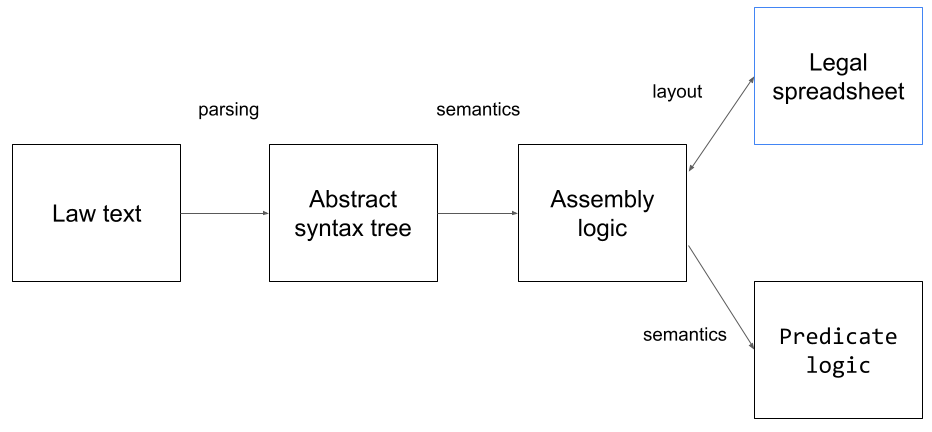
\includegraphics[width=0.8\textwidth]{pipeline.png}
\caption{The pipeline}
\label{pipeline}
\end{figure}

Figure~\ref{pipeline-ex} shows an example of a text at different stages through the pipeline. The rest of this section explains each step of the pipeline in detail.
% J: material merged into the above, but kept the older content in comments for now.
% The pipeline begins by converting statutory text in natural language into abstract syntax tree using

% The starting point of the project presented in this paper was a system consisting of \textbf{spreadsheets} and their translation to logical formulas. The cells of the spreasheet were natural language expressions, which were parsed into syntax trees with the help of a grammar. What was missing from the complete pipeline from text to logic was the conversion from the original text to spreadsheets. This step was made manually, and the focus of the projects was on the later parts of the pipeline. Thus the main contribution of the present paper is to define an automated conversion of texts to spreadsheets.

% The first part of this is a grammar that parses texts to abstract syntax trees. The second part is a conversion to a new intermediate representation between syntax trees, spreadsheets, and logic. We call this representation \textbf{assembly logic}, in analogy to assembly languages in compilers, if we think of spreadsheets and logics as "machine languages", whose long distance to the source language is bridged by the assembly language.

\subsection{Building the Grammars}

Parsing the text is performed by the Grammatical Framework (GF) software \cite{ranta-2011}.
The parser is driven by a grammar, which specifies a relation between strings and abstract syntax trees. In typical GF applications, abstract syntax trees are processed further, usually in translations to other languages but also in logical semantics. GF grammars are usually written by hand, to guarantee a precise correspondance to desired abstract syntax trees. The process is helped by GF's module system and extensive libraries, which reduce the need of manual work to the minimum. This is particularly useful in the most typical application of GF, Controlled Natural Language (CNL) \cite{fuchs-al-2008,angelov-ranta-2009}. In such applications, the language can be made to follow grammar rules defined in the GF Resource Grammar Library (RGL, \cite{ranta-2009}).

However, the RGL does not cover all the constructs in Singaporean law text, which means that some grammar writing needs to be done from scratch. In particular, the text contains indented lists, paragraph numbers, and references, which significant for the logical structure and which we wanted to capture by the parser. In order to make sure to capture everything, we started grammar writing in a data-driven, top-down way, starting from entire lines of text and going forward by stepwise refinements of the grammar rules.

The most efficient way to produce the grammar turned out to be a semi-automatic method consisting of manual annotations from which a script generated GF rules.
\todoj{we need to explain the annotation scheme and show why it might be useful. especially: how can someone other than us do this well? How do we know we have done it well?}

Figure~\ref{grammar-gen} shows an example of a line of a text, the annotations added to it, and the resulting grammar rules.

\begin{figure}
 \begin{framed}
\bequ
\textbf{A line in the text:}
\bequ
\textit{Item (2) without limiting subsection Ref (1)(a), a CN data breach is deemed to VP result in significant harm to an individual —}
\enqu
\textbf{The line annotated with marks for terminals} (\verb6#6) \textbf{and nonterminals} (\verb6*6):
\bequ
\begin{verbatim}
*Item (2) #without #limiting #subsection *Ref (1)(a) #,
#a *CN data breach #is #deemed #to
*VP result in significant harm to an individual #—
\end{verbatim}
\enqu
\textbf{Grammar rules derived by the script:}
\bequ
\begin{verbatim}
Line ::= Item "without" "limiting" "subsection" Ref ","
         "a" CN "is" "deemed" "to" VP "-" ;
Item ::= "(2)" ;
Ref  ::= "(1)(a)" ;
CN   ::= "data" "breach" ;
VP   ::= "result" "in" "significant"
         "harm" "to" "an" "individual" ;
\end{verbatim}
\enqu
\textbf{The last of the grammar rules manually edited by step-wise refinements:}
\bequ
\begin{verbatim}
VP2 ::= "result" "in" NP ;
NP  ::= "significant" "harm" "to" NP ;
NP  ::= "an" CN ;
CN  ::= "individual" ;
\end{verbatim}
\enqu
\textbf{Abstract syntax functions in the resulting GF grammar:}
\bequ
\begin{verbatim}
fun VP2_result_in : VP2 ;
fun CN_significant_harm_to_NP : NP -> CN ;
fun NP_an_CN : CN -> NP ;
fun CN_individual : CN ;
\end{verbatim}
\enqu
\enqu
\end{framed}
\caption{The grammar extraction process.}
\label{grammar-gen}
\end{figure}

The grammar produced by the script is a BNF (context-free) grammar, in a notation that can be used in GF as it is.
Internally, GF adds to each rule abstract syntax functions, whose names are derived from items in the rule itself.
Full GF is more expressive and more abstract than BNF.
In the example of Figure~\ref{grammar-gen}, the full power can be used to merge together the function \verb6CN_individual6 with another derived function \verb6CN_individuals6, to a single function that covers both the singular and the plural form of the noun.
Similarly, the rules \verb6NP_an_CN6 can be merged with \verb6NP_a_CN6.
An advantage, in addition to getting fewer rules, is that the choice of the sinular and the plural, or \textit{a} vs.\ \textit{an}, can then be made precisely depending on the context.

\subsection{Converting the AST to predicate logic}

The pipeline in Figure~\ref{pipeline} branches from Assembly Logic to two directions: to spreadsheets, described in the next section, and to predicate logic, to be discussed here.

The predicate logic step itself is divided to two phases:
\begin{enumerate}
\item Assembly logic is mapped into a many-sorted logic with Russell iota terms.
\item The many-sorted logic is mapped into ordinary predicate logic and rendered in the TPTP notation.
\end{enumerate}
The many-sorted logic is chosen because of its better support of compositional translation.
Thus quanfication expressed by noun phrases (such as \textit{any storage medium}) are compositionally interpreted as quantifiers with sorts, instead of dividing them into unsorted quantiers and sort predicates.
The sorts are eliminated as a part of the conversion from many-sorted to ordinary logic.

Even more crucially, anaphoric expressions (such as \textit{that organization}) are interpreted as definite descriptions formalized as iota terms.
These iota terms are eliminated in a pass that looks for non-iota terms in their context of use.
Figure~\ref{anaphora} shows an examples of this, showing thestructure of ``donkey sentences'' well-known in linguistic literature (\textit{if a man owns a donkey he beats it}) \cite{geach-1962,kamp-1981}
Such a sentence has an existential quantifier in the antecedent, and a pronoun or definite desctiption referring to it in the succedent.
To express this reference in ordinary predicate logic, the existential quantifier is changed into a universal with a wide scope of the implication.

 \begin{figure}
  \begin{framed}
  \bequ
  \textbf{A toy example of a ``donkey sentence'':}
  \bequ
 \textit{if a notification is a data breach , the notification is affected}
 \enqu

 \textbf{Compositional interpretation in many-sorted logic with iota terms:}
 \[
(\exists x : \eop{notification})\eop{data\_breach}(x) \, \supset \, \eop{affected}(\iota(\eop{notification}))
\]

 \textbf{Conversions to ordinary predicate logic in TPTP notation:}
 \bequ
\begin{verbatim}
![X]:(notification(X) => data_breach(X) => affected(X))
\end{verbatim}
 \enqu
 \enqu
   \end{framed}
 \caption{Iota terms are eliminated via anaphora resolution.
 }
\label{anaphora}
\end{figure}

Donkey sentences are ubiquitous in law text, as in many other types of text.
To our surprise, also ``inverted donkey sentences'' occurred in our sample text --- ones in which the existential appears in the succedent and is referred to in the antecedent.
What makes this sound natural is that the whole implication appears in reverse: \textit{a man beats a donkey if he owns it}.
Figure~\ref{donkey}

\begin{figure}
 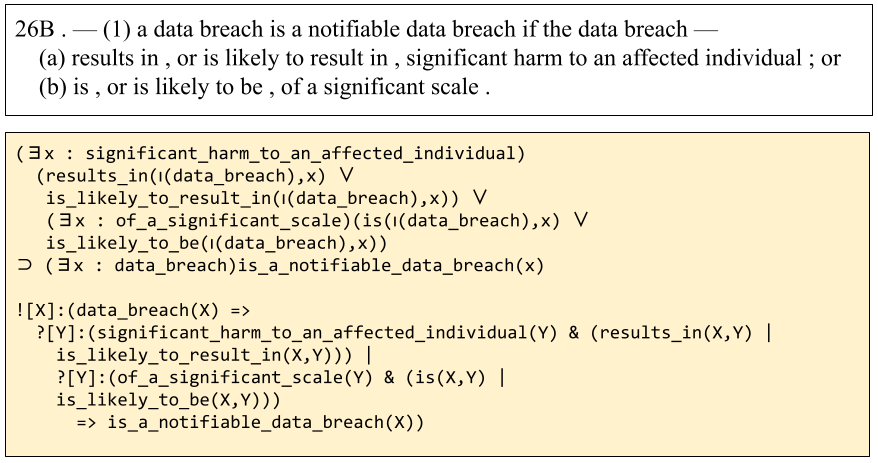
\includegraphics[width=0.96\textwidth]{anaphora.png}
\caption{An inverted donkey sentence from the actual law text.}
\label{donkey}
\end{figure}

\subsection{Visualisation in Spreadsheets}

\todoj{This part on spreadsheets needs to be simplified and shortened if we are to fit it all into 8 pages. I think we can only give max 1 page to this, and it is not the main focus of the paper. Could the Haskell figure be shortened? Those interested can be linked to the actual github code.}

Aside from predicate logic, the AST allowed us to visualise the statute's structure in spreadsheet form. This spreadsheet notation is presently under development by our research team and will be more formally described in a separate paper. Presently, it suffices to note that this visualisation was developed to help non-technical users learn, understand, and write (intermediate) legal formalisms more easily. To this end, it is a quasi-logical visual language where legal operators, predicates, and conclusions are arranged and indented following a particular, controlled syntax...
\todoj{Need Meng to properly summarise this. Please make it short and concise.}

We implemented spreadsheets with a recursive datatype \verb6Box6, where a box consists of a header and cells, where each cell is a box with a title.

This structure supports compositional conversion from a tree-like representation, but also rendering as tab-separated files, which can be read into spreadsheet editors.
Figure~\ref{assembly} shows this type, together with the other concepts related to spreadsheets.

\begin{figure}
  \begin{framed}
  \bequ
  \textbf{The recursive Haskell datatype for spreadsheets:}
 \bequ
\begin{verbatim}
data Box = Box {
   header :: String,
   cells :: [(String, Box)]
  }
\end{verbatim}
 \enqu

 \textbf{Some assembly logic constructors:}
 \bequ
\begin{verbatim}
data Cat =
  CProp | CSet | CInd | -- ...
data Formula =
    Atomic Cat Atom
  | Conjunction Cat ConjWord [Formula]
  | Implication Formula Formula
  | Conditional Formula Formula     -- reverse implication
  | Quantification String Formula   -- quantifier + domain
\end{verbatim}
 \enqu

 \textbf{Semantics of abstract syntax trees in the assembly logic:}
 \bequ
\begin{verbatim}
iNP :: Env -> GNP -> Formula
iNP env np = case np of
  GNP_any_CN cn -> Quantification "ANY" (iCN env cn)
  GNP_each_CN cn -> Quantification "EACH" (iCN env cn)
  -- ...
  _ -> Atomic CInd (lin env (gf np))
\end{verbatim}
 \enqu

 \textbf{Conversions from assembly logic to spreadsheets:}
 \bequ
\begin{verbatim}
formula2box :: Formula -> Box
formula2box formula = case formula of
  Atomic _ a  -> atomBox a
  Implication f g -> ifBox [formula2box f] [formula2box g]
  Quantification s f -> leftsideBox s [formula2box f]
\end{verbatim}
 \enqu
 \enqu
   \end{framed}
 \caption{Data structures and conversions related to spreadsheet and the assembly logic.
 }
\label{assembly}
\end{figure}

\todoj{ This para below reads like it belongs somewhere in the pipeline overview, probably even before the part where we talk about grammars?}
Notice that the ultimate unit of semantic interpretation is a paragraph consisting of several lines. This is the case, for instance with the example in Figure~\ref{pipeline-ex}.
In the current implementation, the parser reads the document line by line, and a separate process is used for segmenting groups of lines into paragraphs.
The reason for this set-up is purely practical: semantic units can be arbitrarily long sequences of lines, and the parser may get slow in such cases.

\section{Formalising the Personal Data Protection Act}
\label{sec:pdpa}

We demonstrate our proposed pipeline on Part 6A the PDPA. Like the EU's \textit{General Data Protection Regulation} (GDPR), the PDPA is Singapore's primary personal data protection statute and prescribes obligations surrounding the collection, use, disclosure, and deletion of personal data. Part 6A in particular stipulates when and how organisations are expected to notify regulators of personal data breaches (e.g.\ a hospital's patient databases are leaked). We chose the PDPA as a case study for three reasons. First, modelling the PDPA was a practical suggestion from the Personal Data Protection Commission (the Commission), Singapore's primary data regulator, based on their experience having to field numerous questions and prepare volumes of public-friendly guidelines on Part 6A. There was thus a clear use case for our technology. Second, while the PDPA has not been examined in prior AI \& Law literature, its subject matter connects it to established work modelling the GDPR \cite{palmirani_modelling_2018, brennan_gdpr_2021, hickey_gdpr_2021}.

Third, the notification sections we examine are sufficiently complex to demonstrate the utility of a computational law approach in general and our pipeline in particular. Counter-intuitively, organisations are not always expected to immediately disclose data breaches upon discovering them. Rather, breaches are only notifiable if they (are likely to) result in significant harm affected individual(s), or if they are of ``significant scale'' (PDPA s 26B(1)). If so, there is a general duty to report the breach to the Commission ``as soon as practicable'' (s 26D(1)). The organisation must thereafter notify each affected individuals ``in any manner that is reasonable in the circumstances'' (s 26B(2)) --- unless the Commission directs them not to (s 26D(2)). The Commission's published guidelines explain that this may be directed if the breach is of such severity that public responses to it may need to be carefully managed
 \todoj{ Meng please confirm and provide a cite}.
 Modelling these rules allowed us to surface the implicit race condition between notifying the Commission and the affected individuals: an organisation which proactively informed both groups at the same time might inadvertently flout the statute's design.

\todoj{Might remove this table if we need space, doesn't add that much}
Table \ref{stats} provides a statistical summary of the primary input text.

[TODO (AR): At the time of writing, the final translation to logic fails for two logical units, and the logic rules require better verification.]

\begin{table}
  \begin{tabular}{|l|r|}
\hline
lines & 66 \\
characters & 6154 \\
tokens & 1072 \\
unique tokens & 229 \\
tokens per line on average & 16 \\
tokens on the longest line & 56 \\
logical units & 46 \\
\hline
  \end{tabular}
  \caption{Statistics about Personal Data Protection Act (PDPA), Part 6A}
  \label{stats}
\end{table}

To formalise Part 6A, we first...
 \todoj{ can someone write a one para summary of the actual process here? That is, how exactly did we convert Part 6A into code? How did we build the specific grammars, etc?}
  Next, we... Finally, ...

Figure \ref{pipeline-ex} illustrates selected portions of the text through various stages of the pipeline.

\begin{figure}
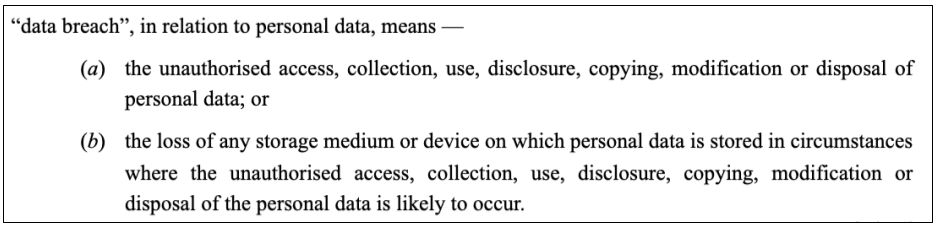
\includegraphics[width=0.8\textwidth]{text.png}
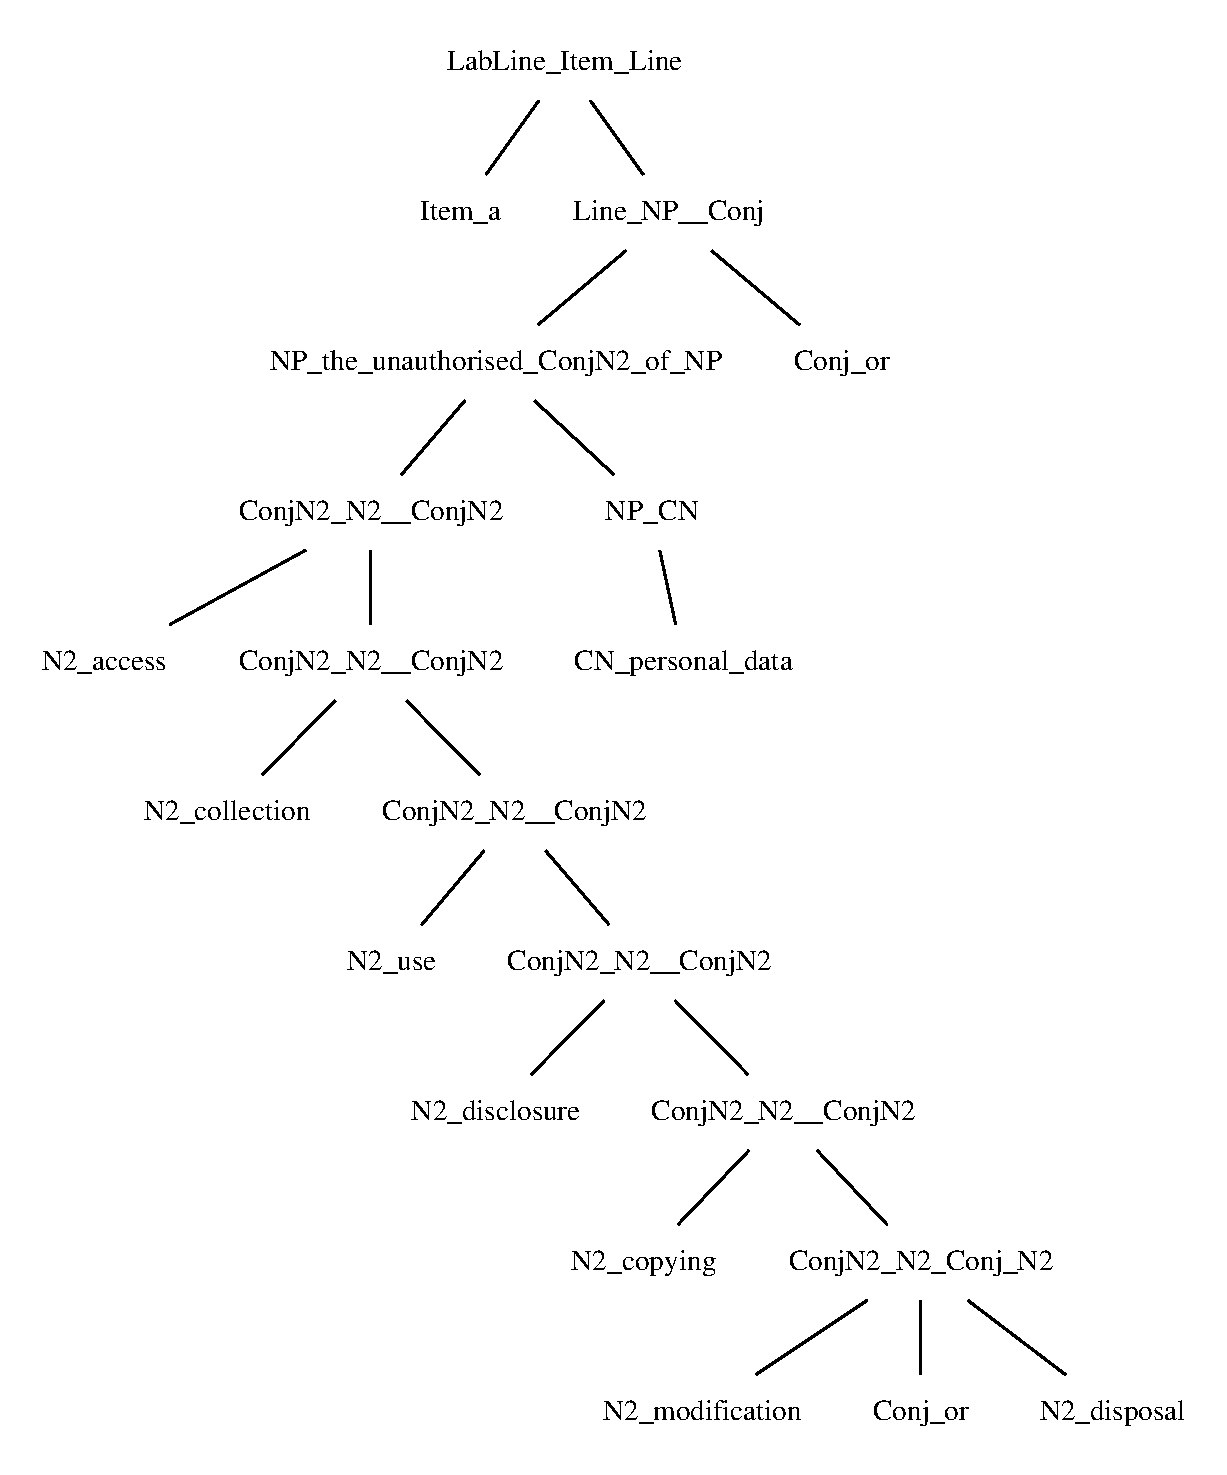
\includegraphics[width=0.4\textwidth]{tree.eps}
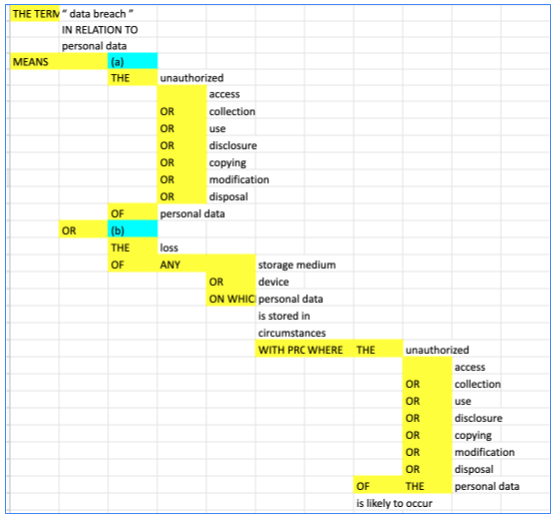
\includegraphics[width=0.6\textwidth]{assembly.png}
\small
\begin{verbatim}
![X]:(data_breach(X) & ?[Y]:(personal_data(Y) & IN_RELATION_TO(X,Y)) <=>
(personal_data(X) & ?[Y]:((access(Y,X) | collection(Y,X) | use(Y,X) |
disclosure(Y,X) | copying(Y,X) | modification(Y,X) | disposal(Y,X)) &
unauthorized(Y))) | (((storage_medium(X) | device(X)) & (personal_data(X) &
?[Y]:((circumstances(Y) & (((unauthorized(Y) & (access(Y) | collection(Y) |
use(Y) | disclosure(Y) | copying(Y) | modification(Y) | disposal(Y))) &
is_likely_to_occur(Y))) & is_stored_in(X,Y)))) & loss(X))))
\end{verbatim}
\normalsize
\caption{An example through the pipeline: text, abstract syntax tree (of the second line), spreadsheet, and formula in TPTP notation.
TODO (AR): the TPTP formula is not quite correct - I will have to fix the semantics.
}
\label{pipeline-ex}
\end{figure}

\section{Discussion and future work}
\label{sec:future}

\todoj{ We will need to offer some insights on how well the thing worked. How did we know if we got a good logical output? Were there any standards we checked it against?}

The most important tasks for future work are to link this pipeline with the previous work at CCLAW, which have much more precision and detail: the spreadsheets and the grammar of smaller units.

As regards spreadsheets, and in fact the interpretation in logic, the current experiment is simple-minded in the sense that it only looks at the document at hand.
The real spreadsheets also take into account other documents that affect the interpretation, and show this information in the spreadsheets.

As for the grammar, the bulk of the work will be in the detailed structure of noun phrases and predicates that appear in single cells.
It also remains to see how much of the line and paragraph structures is already included in the grammar based on the sample, but the variation there can be expected to be numerically smaller.

We do not claim to have solved the natural language barrier. But given the tedium which necessarily accompanies manual translations of law to logic, the advent of such software would accelerate research and development of computational law systems, even if the algorithms' outputs were, realistically speaking, not perfectly faithful to original law and thus required manual vetting.

\bibliographystyle{plain}
\bibliography{complaw-bib}

\end{document}